\begin{figure}[t!]
  \begin{center}
    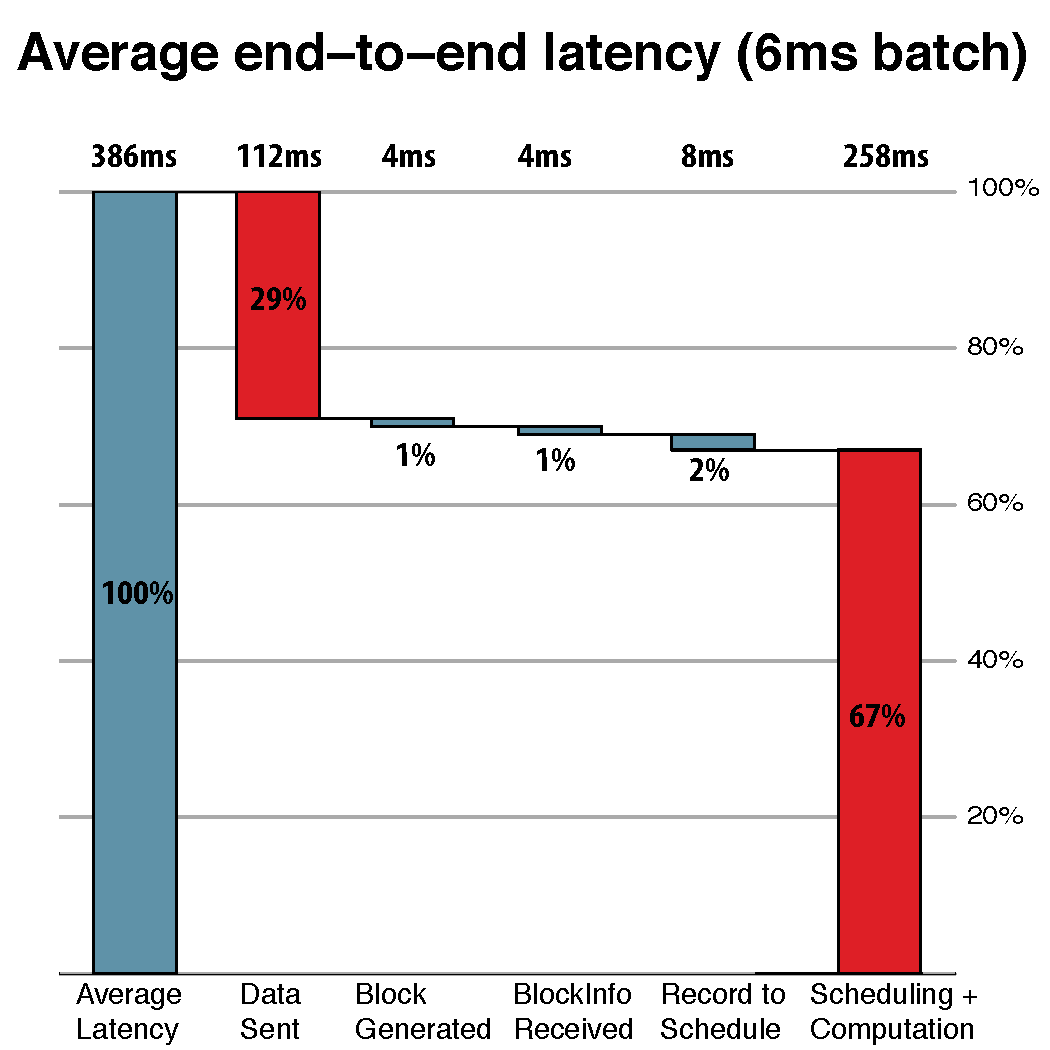
\includegraphics[scale=0.40]{images_graphs/waterfall/6ms_time_breakdown.pdf}
  \end{center}
  \caption{}
  \label{fig:SparkStreaming_time_breakdown}
\end{figure}

To better understand the performance and limitations of Spark Streaming we conducted a benchmark study of the system. 

To this end we used a synthetic workload to exercise Spark Streaming and measure how the system behaves under different scenarios. 
The application consists of a simple transformation of a stream of 25-byte text records.
In this benchmark we do not focus on the time spent during computation.
First, the computation time is almost always orthogonal to the architecture used.
Secondly, there is other work aimed at improving computation times in streaming or Map-reduce systems.
%    There is parallel work on improving the performance of streaming computations that can be used to improve the execution times of tasks.

To run this benchmark we have deployed a receiver and a record generator in two different machines in the same cluster. 
The record generator generates as many 25-byte records as necessary to achieve a user-specified throughput. 
Each record contains a timestamp that corresponds to the moment of creation of the record. 
The receiver uses the Spark Streaming API to consume this data. 
A task is generated periodically, according to a user-defined frequency, and scheduled to a node where the data is processed.

We have instrumented the code of Spark Streaming to record the time at which the record transitions a phase (e.g., a task to process a record is scheduled).
%#understand how much time each record stays on each phase of the streaming process.
This allows us to gather 1) the time each record spends on each phase of the streaming process, 
and 2) the time between the generation of each record and the moment of computation -- end-to-end latency.


%When processing records, the time between the generation of each record and the moment of computation is captured. 
%We refer to this value throughout the paper as the end-to-end latency. 

The results of the first experiment we conducted is captured in Figure~\ref{fig:Batchsize_vs_latency}.
In this graph we show the average end-to-end latency obtained when running Spark Streaming with different batch windows and throughputs. 
Changing the batch window configuration allows us to tune the responsiveness of the system; a lower value means that each records spends less time in memory waiting for a task
to be spawned in order to process that same record. 
Varying the number of records generated by the stream source (throughput), allows us to understand how 
Spark behaves when it has to do more/less work per unit of time and how that affects latency.

In the graph we see that for a throughput value of 10Mb/sec Spark.


\begin{figure}[t!]
  \begin{center}
    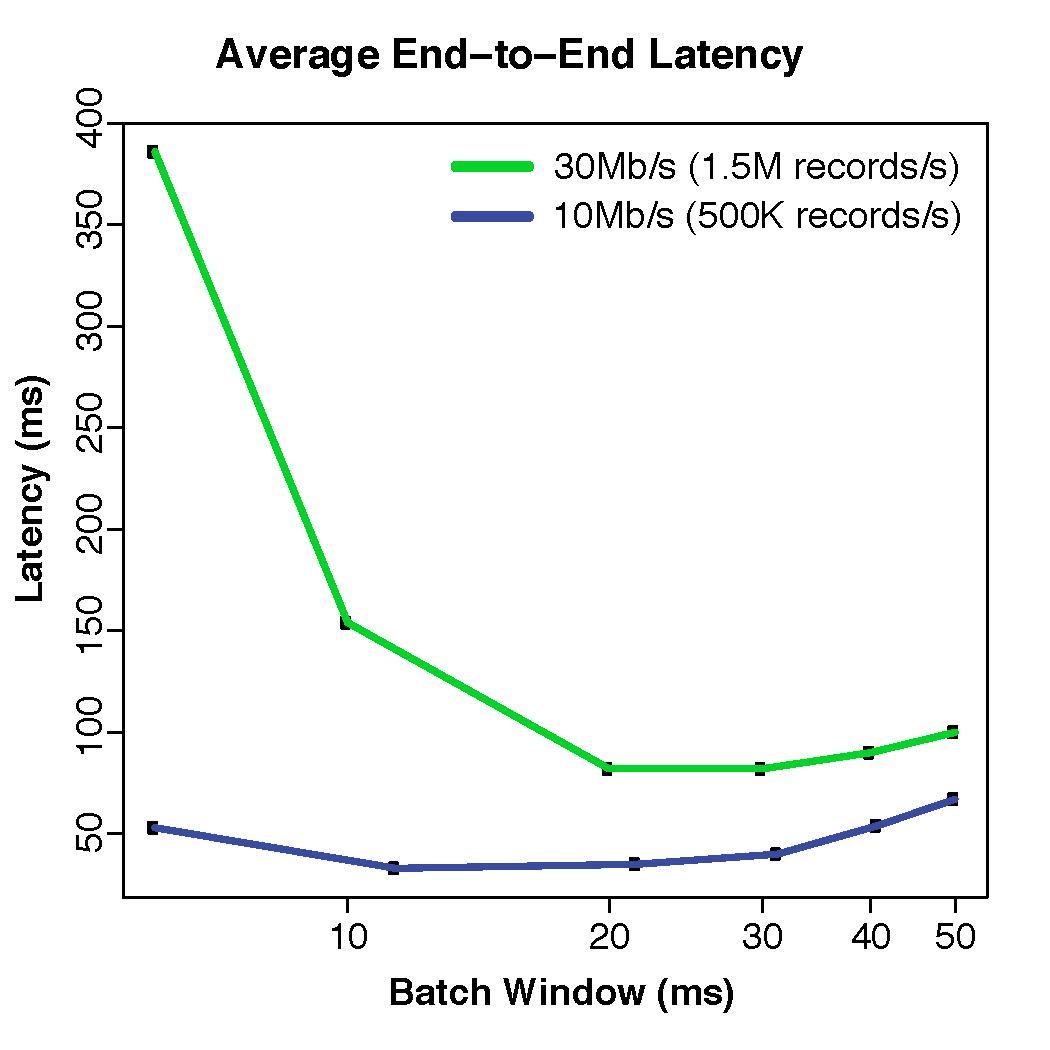
\includegraphics[scale=0.35]{images_graphs/batchsize_vs_latency/batchsize_vs_latency3.pdf}
  \end{center}
  \caption{}
  \label{fig:Batchsize_vs_latency}
\end{figure}

%%
%%\subsection{Scheduling Scalability}
%%
%%A significant amount of work has been done on scheduling. Many contributions aim to develop schedulers that can provide guarantees like fairness or utilization of resources~\cite{}. Others focus on making the schedule scale and/or provide low-latency scheduling of tasks~\cite{Sparrow, CFS}.
%%
%%During the execution of a Spark Streaming application, the Driver (a central component of Spark) generates tasks periodically and adds them to the tail of a scheduling queue. This queue is continuously probed by the scheduler, which schedules by taking tasks from the queue and sending them to worker nodes for processing.
%%As applications specify lower batch intervals to process results more quickly, the number of tasks added to the queue per unit of time increases. Eventually, the scheduler will be unable to keep up with the rate of tasks being added to the queue. This results in an indefinite increase in the average time to schedule a task, which is worse considering the fact that tasks in one batch have less time to be processed before the next batch is generated.
%%From this observation, we can see that lower batch intervals lead to lower task latencies, less throughput and more tasks scheduled per second. On the other hand, larger batch intervals lead to higher throughput, higher task latencies and less tasks scheduled per second. 
%%
%%To understand the performance of the current version of Spark Streaming, we have benchmarked the end-to-end latencies of tasks with different batch intervals. 
%%Our benchmarks were run on a 16-node cluster, with each node having 16 cores. We have used 120 receivers on 4 nodes. 
%%With this configuration, Spark Streaming generates 120$*$1000/(batch interval) tasks per second.
%%Because we are solely interested in benchmarking the scheduling performance, we ran applications that generate no-op tasks.
%%
%%We have found that for a batch interval less than 40ms the system becomes unstable because the scheduler cannot keep up with the rate of tasks generated. This instability leads to increasingly higher scheduling delays and increasing garbage collection activity due to higher memory usage. \joao{Need a graph here showing end-to-end latency of tasks with varying batch intervals}
%%
%%\subsection{Network Overhead}
%%As the number of tasks increases, so does the amount of communication between the driver and executors. We plan to increase the network throughput using InfiniBand, and also explore using RDMA to realize zero-copy. Ideally with these improvements, not only network communication will be faster, the driver will also have more CPU time to schedule tasks, ultimately reducing the latencies of running tasks.
%%
